% XeLaTeX

\documentclass[a4paper]{article}
\usepackage{ctex}
\usepackage{xypic}
\usepackage{amsfonts,amssymb}
\usepackage{multirow}
\usepackage{geometry}
\usepackage{graphicx}
\usepackage{listings}
\usepackage{lipsum}
\usepackage{courier}
\usepackage{fancyvrb}
\usepackage{etoolbox}


\linespread{1.2}
\geometry{left=3cm,right=2.5cm,top=2.5cm,bottom=2.5cm}

\makeatletter
\patchcmd{\FV@SetupFont}
  {\FV@BaseLineStretch}
  {\fontencoding{T1}\FV@BaseLineStretch}
  {}{}
\makeatother

\lstset{basicstyle=\small\fontencoding{T1}\ttfamily,breaklines=true}
\lstset{numbers=left,frame=shadowbox,tabsize=4}
%\lstset{extendedchars=false}
\begin{document}

\title{实验九 \ 在FAT12盘结构中引导操作系统 \ 实验报告}
\author {数据科学与计算机学院 \ 计算机科学与技术 2016 级 \\ 王凯祺 \ 16337233}
\maketitle

\section{实验目的}

\begin{itemize}
\item 了解 FAT12 磁盘结构
\item 会创建 FAT12 格式的软盘
\item 会从 FAT12 格式的磁盘中寻找文件、复制文件到内存
\end{itemize}

\section{实验要求}

\begin{itemize}
\item 用C语言+汇编语言编写一个程序,编译产生一个COM格式的可执行程序,用于显示一个FAT12的BPB和EBPB内容。这个程序作为一个用户程序,保存在你的映像文件中的FAT12文件系统中。
\item 用C语言+汇编语言编写一个程序,编译产生一个COM格式的可执行程序,用于列出一个FAT12的根目录中所有文件信息,如文件名、文件大小、文件创建日期等等。这个程序作为一个用户程序,保存在你的映像文件中的FAT12文件系统中。
\item 修改你的操作系统原型3,将内核执行体用一个文件形式存放在映像盘中,同时按FAT12盘格式的要求,修改引导程序,从FAT12根目录中加载内核。
\item 修改内核程序,实现用命令行从FAT12中加载任意一个用户程序。
\end{itemize}

\section{实验步骤}

\subsection{了解 FAT12 磁盘结构}

看了老师提供的资料,我是一脸懵的。我需要弄懂几个问题:

\begin{itemize}
\item FAT1 和 FAT2 是什么?它有什么用?
\item 簇是什么?软盘中的簇有多大?
\item 文件是如何存储的?
\end{itemize}

为此,我特意用 Windows XP 加载一张空的软盘镜像,并格式化。

\newpage

\begin{figure}[!hbp]
\centering
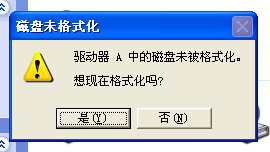
\includegraphics[scale=0.5]{pics/1.png}
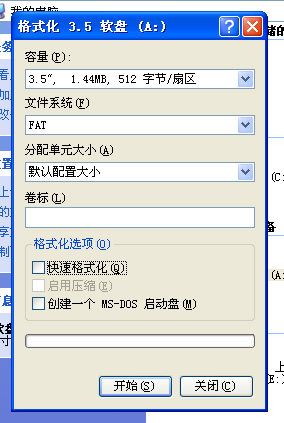
\includegraphics[scale=0.5]{pics/2.png}
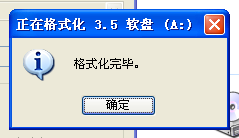
\includegraphics[scale=0.5]{pics/3.png}
\end{figure}

我们可以看到,在第一个扇区, Windows 为这个软盘写了 BPB 和 EBPB 信息,并写了一个操作系统进去(功能是显示两句话~)!

\begin{figure}[!hbp]
\centering

\includegraphics[scale=0.5]{pics/4.png}
\end{figure}

\newpage

\begin{figure}[!hbp]
\centering
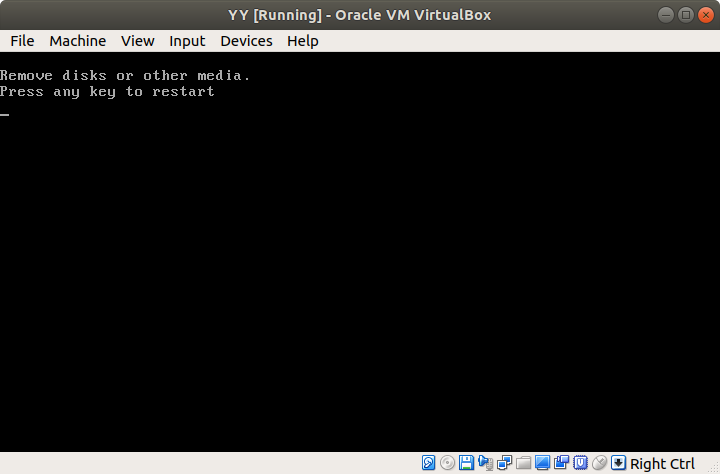
\includegraphics[scale=0.5]{pics/5.png}
\end{figure}

然后我往里面写了三个文件,分析 FAT 表结构。

我发现 FAT1 和 FAT2 是一样的,一个位于第 2 扇区(偏移地址 0x0200),一个位于第 10 扇区(偏移地址 0x1400),我使用 Google 搜索后,知道他们是主要 FAT 表和备份 FAT 表的关系。FAT 表存储的是下一个簇放在什么地方。每个文件可以看成是一条链表,一直指到 0xFFF 表示结束。

\begin{figure}[!hbp]
\centering
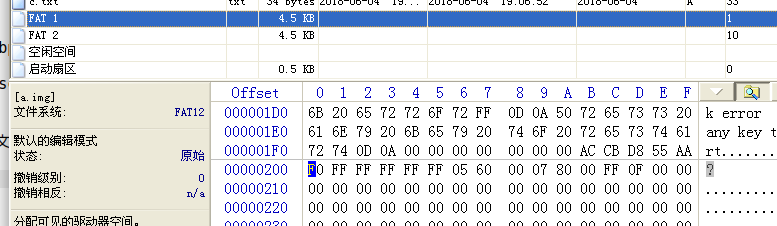
\includegraphics[scale=0.5]{pics/6.png}
\end{figure}

根目录的文件摘要信息存储在第 20 - 33 扇区(偏移地址 0x2600 - 0x41FF),每个文件的摘要占 32 字节,格式 PPT 已经说得很清楚啦!

\begin{figure}[!hbp]
\centering
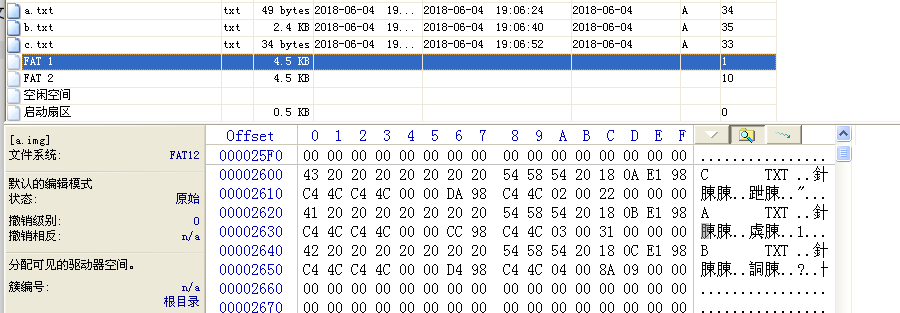
\includegraphics[scale=0.5]{pics/7.png}
\end{figure}

通过对大文件的分析,我知道一簇是 512 字节。

了解好这些之后,可以开始写代码啦 :)

\subsection{编写引导扇区程序}

这一部分是本实验中最最最最最难的!为什么这样说?我们先来了解一下需要干什么。

\begin{itemize}
\item 复制 FAT 表到内存
\item 在根目录寻找 LOADER.COM 
\item 找到 LOADER.COM 的起始簇号
\item 根据簇号计算磁头号、柱面号、扇区号
\item 复制扇区
\item 根据该簇号在 FAT 表寻找下一簇号
\end{itemize}

而这一切,都必须在 448 字节以内(512 字节扣去 "55AA" 的 2 字节、BPB 和 EBPB 的 62 字节)完成,多一个都不行!

而且,更要命的是,这不同于操作系统内核可以用 C 语言实现,这里的所有的代码都必须用汇编写。由此可见,这次项目的工作量非常非常大。

\paragraph{BPB 和扩展 BPB}

这部分代码照抄老师的,把 OEMName 和序列号等个性化信息改成了我的。

\begin{lstlisting}[language={[x86masm]Assembler}]
org  7c00h		; BIOS将把引导扇区加载到0:7C00h处,并开始执行

	jmp short Start                      ; Jump, 2 Bytes
	nop                                  ; 1 Bytes
	BS_OEMName DB 'AM-OS9.0'             ; OEM String, 8 Bytes
	BPB_BytsPerSec DW 512
	BPB_SecPerClus DB 1
	BPB_RsvdSecCnt DW 1
	BPB_NumFATs DB 2
	BPB_RootEntCnt DW 224
	BPB_TotSec16 DW 2880
	BPB_Media DB 0xF0
	BPB_FATSz16 DW 9
	BPB_SecPerTrk DW 18
	BPB_NumHeads DW 2
	BPB_HiddSec DD 0
	BPB_TotSec32 DD 0
	BS_DrvNum DB 0
	BS_Reserved1 DB 0
	BS_BootSig DB 29h
	BS_VolID DD 16337233h
	BS_VolLab DB 'AM-OS 9.0  '           ; 11 Bytes
	BS_FileSysType DB 'FAT12   '         ; 8 Bytes
\end{lstlisting}

\paragraph{定义常量}

为了避免硬编码,我定义了以下常量。

\begin{lstlisting}[language={[x86masm]Assembler}]
FATMem equ 2000h         ; FAT 分区表保存的段地址
KernelCS equ 0a00h       ; 加载内核的段地址
KernelIP equ 0100h       ; 加载内核的偏移地址
                         ; 内核加载在 0xA100
\end{lstlisting}

\paragraph{复制 FAT 分区表到内存指定位置}

此部分代码将软盘的前 33 个扇区(包括引导扇区、FAT1、FAT2和根目录文件摘要)拷贝到 FATMem ($= 0x2000$) 处。

\begin{lstlisting}[language={[x86masm]Assembler}]
Start:
                                       
LoadFAT:
	;读软盘或硬盘上的若干物理扇区到内存的ES:BX处:
	mov word bx, FATMem
	mov es, bx
	xor bx, bx
	mov ah,2                 ; 功能号
	mov al,33                ;扇区数
	mov dl,0                 ;驱动器号 ; 软盘为0,硬盘和U盘为80H
	mov dh,0                 ;磁头号 ; 起始编号为0
	mov ch,0                 ;柱面号 ; 起始编号为0
	mov cl,1                 ;起始扇区号 ; 起始编号为1
	int 13H ;                调用读磁盘BIOS的13h功能
	; FAT 根目录已加载到指定内存区域 0x2000:0x0000 中
\end{lstlisting}

\paragraph{在根目录查找内核并返回首簇地址}

这部分代码就比较复杂了。这一共两层循环,外层循环是 0 - 223 ,表示遍历到根目录的第几个文件,内层循环则是做字符串匹配,若某个文件的文件名匹配 “LOADER  COM” 能成功,则将该摘要中的首簇号提取出来,放在 dx 寄存器中。

\begin{lstlisting}[language={[x86masm]Assembler}]
getFAT:
;  Output: if LOADER.COM found in [file_num], return dx = [start sector], bx = [size]
;          otherwise, dx = 0
	
	xor dx, dx                 ; dx = 0
	mov ax, 2600h
	xor cx, cx                 ; cx = 0
	
FATfindLoop:
	xor bx, bx
	mov ds, bx
	mov [axbak], ax
	push ax
	push cx
	mov ax, KernelStr          ; ax = addr("KERNEL  BIN")
	xor cx, cx                 ; cx = 0
	
KernelStrMatch:
	push ax
	xor ax, ax
	mov ds, ax
	mov bx, [axbak]
	mov ax, FATMem
	mov ds, ax
	pop ax
	add bx, cx                 ; the cx-th bit
	mov bl, [bx]
	push ax
	xor ax, ax
	mov ds, ax
	mov byte [char1], bl
	pop ax

	mov bx, ax
	mov bl, [bx]	
	cmp bl, [char1]
	jnz KernelNotMatch
	
	inc ax
	inc cx
	cmp cx, 11
	jb KernelStrMatch
	xor bx, bx
	mov ds, bx
	mov dx, [axbak]            ; matched, dx = kernel addr
KernelNotMatch:
	
	pop cx
	pop ax
	add ax, 20h
	inc cx
	cmp dx, 0
	jnz KernelOK
	cmp cx, 224
	jb FATfindLoop
	call dispStr
	jmp $
	
KernelOK:
	; dx = kernel addr
	call dispStr
	add dx, 1ah
	mov bx, dx
	mov ax, FATMem
	mov ds, ax
	mov dx, [bx]                ; dx = first cluster
	
	mov ax, KernelIP
\end{lstlisting}

\paragraph{复制扇区}

这个难点就在于磁头号、柱面号、扇区号的计算了。查阅了《软盘结构(磁头号和起始扇区的计算方法)》(https://blog.csdn.net/littlehedgehog/article/details/2147361)后,就能计算出正确的磁头号、柱面号、扇区号,正确地加载指定扇区到指定内存啦!

\begin{lstlisting}[language={[x86masm]Assembler}]
copy_sector:
; Input: dx = cluster number
;        ax = memory offset
;        (KernelCS is DS)
	push ax
	push dx
	xor bx, bx
	mov ds, bx
	mov word [axbak], ax
	add dx, 31
	mov ax, dx
	xor dx, dx
	mov cx, 18
	div cx
	inc dx
	mov byte [qishishanqu], dl
	xor dx, dx
	mov cx, 2
	div cx
	mov byte [citou], dl
	mov byte [zhumian], al
	mov ax, KernelCS
	mov es, ax
	mov bx, [axbak]
	mov cl, [qishishanqu]
	mov ah, 2
	mov al, 1
	mov dl, 0
	mov dh, [citou]
	mov ch, [zhumian]
	int 13h
	
	pop dx
	pop ax
	ret
\end{lstlisting}

\paragraph{寻找下一簇}

在查FAT表时,首先要分簇号的奇偶两种情况来讨论。

记当前簇号为 $x$ , $t_a = \lfloor 3x / 2 \rfloor$, $t_b = t_a + 1$ , $d_a$ 为第 $t_a$ 字节的数据, $d_b$ 为第 $t_b$ 字节的数据。

我对着 FAT 表观察了很久,总结出规律:对于偶簇,选 $d_a$ 的全部 8 位作为低位和 $d_b$ 的低 4 位作为高位组成 12 位整数;对于奇簇,选 $d_a$ 的高 4 位作为低位和 $d_b$ 的全部 8 位作为高位组成 12 位整数。那么这个 12 位整数就是下一簇。

由于涉及分类讨论和位运算操作,这个地方特别难写,也特别难调试。我使用 bochs 一步步跟踪,确认寄存器的值。最后发现是因为奇簇算错了,导致扇区复制错了……

\begin{lstlisting}[language={[x86masm]Assembler}]
find_next_sector:
; Input: dx = cluster number
; Output: dx = next cluster number
	push ax
	mov bx, FATMem
	mov ds, bx
	mov ax, dx
	mov bx, dx
	xor dx, dx
	mov cx, 3
	mul cx
	mov cx, 2
	div cx
	add ax, 200h
	xor dx, dx
	test bx, 1h
	jnz odd_num
	; even_number
	mov bx, ax
	mov dl, [bx]
	inc bx
	mov dh, [bx]
	and dh, 0fh
	jmp even_odd_all_ok
odd_num:
	; odd number
	mov bx, ax
	mov dl, [bx]
	inc bx
	mov dh, [bx]
	shr dl, 4
	mov cl, dh
	and cl, 0fh
	shl cl, 4
	add dl, cl
	shr dh, 4
even_odd_all_ok:
	pop ax
	ret
\end{lstlisting}

\paragraph{跳转内核}

写个循环搬内核到内存,读到 FF8 - FFF 文件结束信号就可以收工,跳转至内核啦!

\begin{lstlisting}[language={[x86masm]Assembler}]
go_and_fetch:
	call copy_sector
	call find_next_sector
	add ax, 200h
	cmp dx, 0ff8h
	jb go_and_fetch
	
	mov ax, KernelCS
	mov bx, KernelIP
	shl ax, 4
	add bx, ax
	jmp bx
\end{lstlisting}

编写好引导扇区后,把未经修改的 LOADER.COM 通过 Windows XP 拖进软盘就能引导啦!

\begin{figure}[!hbp]
\centering
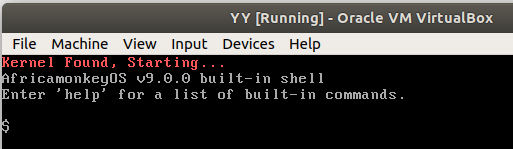
\includegraphics[scale=0.5]{pics/8.png}
\end{figure}

\subsection{修改内核}

由于之前用户程序是按照别的方式从软盘读到内存,现在更换为 FAT12 文件系统,内核在读取用户程序时也需要作出相应的修改。

具体修改的地方:

\begin{itemize}
\item 修改寻找用户程序的函数(从根目录区域搜索),返回值为首簇
\item 新增查找下一簇的函数
\item 修改复制用户程序的函数(由复制连续的好几个扇区改为每次只复制一扇区并查找下一扇区)
\end{itemize}

由于上述的功能在前面引导扇区用汇编写过了,我用 C 语言写当然是毫不费劲啦!

这样,内核就可以加载程序啦!

\paragraph{测试时间片轮转功能}

下面测试的是实验六实现的时间片轮转功能,功能正常。

\begin{figure}[!hbp]
\centering
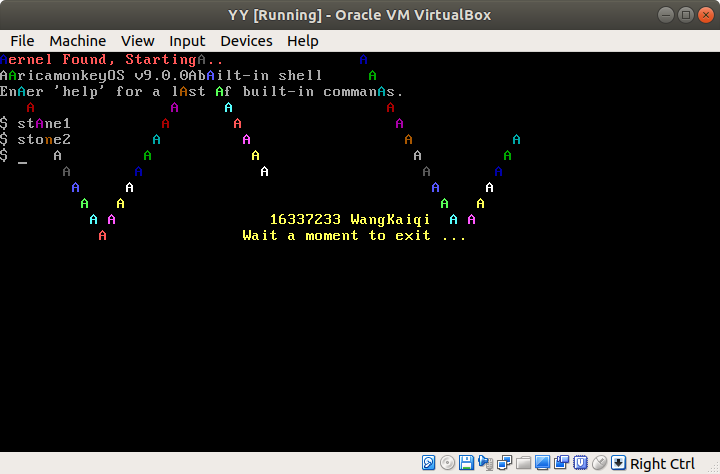
\includegraphics[scale=0.5]{pics/9.png}
\end{figure}

\paragraph{测试 fork 功能}

下面测试的是实验七实现的 fork 功能,功能正常。

\begin{figure}[!hbp]
\centering
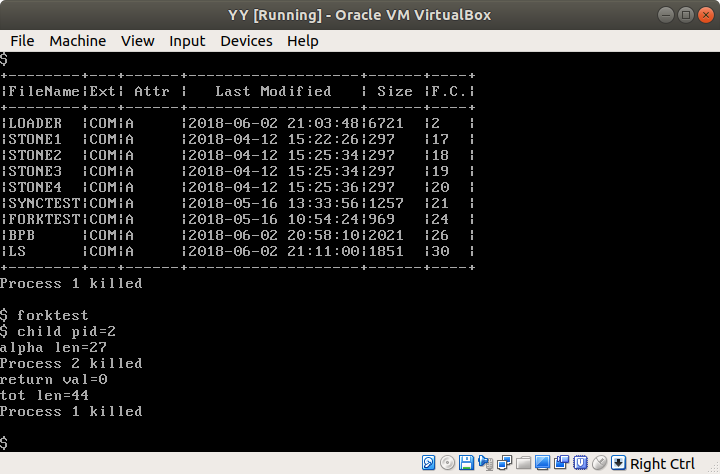
\includegraphics[scale=0.5]{pics/10.png}
\end{figure}

\paragraph{测试信号量功能}

下面测试的是实验八实现的信号量功能,功能正常。

\begin{figure}[!hbp]
\centering
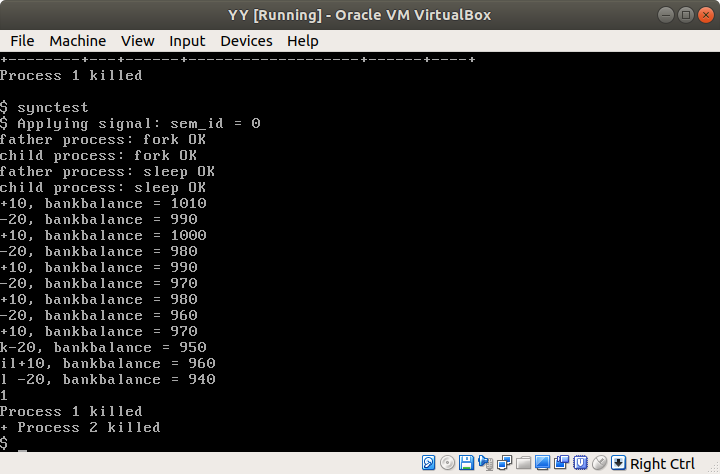
\includegraphics[scale=0.5]{pics/11.png}
\end{figure}

\subsection{编写显示 BPB 和 EBPB 内容的程序}

由于引导扇区程序已经将软盘的前 33 个扇区都加载到 0x2000 段中,这个用户程序就不用再做同样的操作了,直接开始解释 BPB !

\begin{lstlisting}[language=C]
#include "stdlib.h"
#include "stdio.h"

void bpbmain() {
	unsigned char st[0x40], tmp;
	int i;
	for (i = 0; i < 0x40; ++i) {
		asm mov bx, i
		asm push ds
		asm mov ax, 2000h                /* FAT table */
		asm mov ds, ax
		asm mov al, [bx]
		asm pop ds
		asm mov tmp, al
		st[i] = tmp;
	}
	puts("--- BPB Info ---");
	puts_no_new_line("OEM Name: ");
	for (i = 0; i < 8; ++i) putchar(st[i + 0x03]);
	puts("");
	puts_no_new_line("Bytes per sector: ");
	i = (int)st[0x0b] + (((int)st[0x0c]) << 8);
	printint(i);
	puts_no_new_line("Sectors per cluster: ");
	printint((int)st[0x0d]);
	puts_no_new_line("Reserved sector count: ");
	i = (int)st[0x0e] + (((int)st[0x0f]) << 8);
	printint(i);
	puts_no_new_line("Number of file allocation tables: ");
	printint((int)st[0x10]);
	puts_no_new_line("Maximum number of root directory: ");
	i = (int)st[0x11] + (((int)st[0x12]) << 8);
	printint(i);
	puts_no_new_line("Total sectors: ");
	i = (int)st[0x13] + (((int)st[0x14]) << 8);
	printint(i);
	puts_no_new_line("Sectors per File Allocation Table: ");
	i = (int)st[0x16] + (((int)st[0x17]) << 8);
	printint(i);
	puts_no_new_line("Sectors per track: ");
	i = (int)st[0x18] + (((int)st[0x19]) << 8);
	printint(i);
	puts_no_new_line("Number of heads: ");
	i = (int)st[0x1a] + (((int)st[0x1b]) << 8);
	printint(i);
	puts_no_new_line("Hidden sectors: ");
	i = (int)st[0x1c] + (((int)st[0x1d]) << 8);
	printint(i);
	puts("");
	puts("--- EBPB Info ---");
	puts_no_new_line("Physical drive number: ");
	printint((int)st[0x24]);
	puts_no_new_line("Extended boot signature: ");
	printhex((int)st[0x26]);
	puts_no_new_line("Volume serial number: ");
	printhex_no_new_line_no_0x(st[0x2a] >> 4);
	printhex_no_new_line_no_0x(st[0x2a] & 15);
	printhex_no_new_line_no_0x(st[0x29] >> 4);
	printhex_no_new_line_no_0x(st[0x29] & 15);
	puts_no_new_line("-");
	printhex_no_new_line_no_0x(st[0x28] >> 4);
	printhex_no_new_line_no_0x(st[0x28] & 15);
	printhex_no_new_line_no_0x(st[0x27] >> 4);
	printhex_no_new_line_no_0x(st[0x27] & 15);
	puts("");
	puts_no_new_line("Volume label: ");
	for (i = 0; i < 11; ++i) putchar(st[i + 0x2B]);
	puts("");
	puts_no_new_line("File-system type: ");
	for (i = 0; i < 8; ++i) putchar(st[i + 0x36]);
	puts("");
}
\end{lstlisting}

\newpage

结果如下:

\begin{figure}[!hbp]
\centering
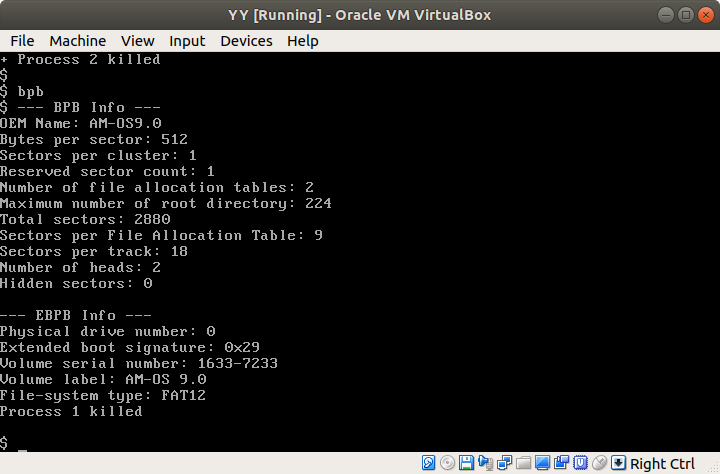
\includegraphics[scale=0.5]{pics/12.png}
\end{figure}

\subsection{编写显示文件摘要的程序}

这个程序列举文件系统根目录所有文件的摘要,包括文件名、扩展名、属性、修改时间、大小、首簇号。

这程序用 C 写,也非常好写。至少比引导扇区的汇编好多了!

\begin{lstlisting}[language=C]
#include "stdlib.h"
#include "stdio.h"

void lsmain() {
	int i, j, k, offset;
	unsigned int t1, t2;
	unsigned char st[32], tmp;
	puts("");
	puts("+--------+---+------+-------------------+------+----+");
	puts("|FileName|Ext| Attr |   Last Modified   | Size |F.C.|");
	puts("+--------+---+------+-------------------+------+----+");
	for (i = 0; i < 224; ++i) {
		for (j = 0; j < 0x20; ++j) {
			offset = 0x2600 + i * 0x20 + j;
			asm mov bx, offset
			asm push ds
			asm mov ax, 2000h                /* FAT table */
			asm mov ds, ax
			asm mov al, [bx]
			asm pop ds
			asm mov tmp, al
			st[j] = tmp;
		}
		if (st[0] == 0x00) continue; /* Empty  entry */
		if (st[0] == 0xe5) continue; /* Erased entry */
		putchar('|');
		for (j = 0; j < 8; ++j) putchar(st[j]);
		putchar('|');
		for (j = 8; j < 11; ++j) putchar(st[j]);
		putchar('|');
		tmp = st[11];
		k = 0;
		if (tmp & 0x01) putchar('R'), ++k;
		if (tmp & 0x02) putchar('H'), ++k;
		if (tmp & 0x04) putchar('S'), ++k;
		if (tmp & 0x08) putchar('V'), ++k;
		if (tmp & 0x10) putchar('D'), ++k;
		if (tmp & 0x20) putchar('A'), ++k;
		for (j = k; j < 6; ++j) putchar(' ');
		putchar('|');
		t1 = st[0x18];
		t2 = st[0x19];
		t1 = t2 << 8 | t1;
		t2 = t1 & 511;
		t1 >>= 9;
		t1 += 1980;
		printint_zero_format(t1, 4);
		putchar('-');
		t1 = t2 >> 5;
		t2 &= 31;
		printint_zero_format(t1, 2);
		putchar('-');
		printint_zero_format(t2, 2);
		putchar(' ');
		t1 = st[0x16];
		t2 = st[0x17];
		t1 = t2 << 8 | t1;
		t2 = t1 & 2047;
		t1 >>= 11;
		printint_zero_format(t1, 2);
		putchar(':');
		t1 = t2 >> 5;
		t2 &= 31;
		printint_zero_format(t1, 2);
		putchar(':');
		t2 *= 2;
		printint_zero_format(t2, 2);
		putchar('|');
		t1 = st[0x1e];
		t2 = st[0x1f];
		if (t1 || t2) {
			puts_no_new_line("65535+");
		} else {
			t1 = st[0x1c];
			t2 = st[0x1d];
			t1 = t2 << 8 | t1;
			printint_format(t1, 6);
		}
		putchar('|');
		t1 = st[0x1a];
		t2 = st[0x1b];
		t1 = t2 << 8 | t1;
		printint_format(t1, 4);
		putchar('|');
		puts("");
	}
	puts("+--------+---+------+-------------------+------+----+");
}
\end{lstlisting}

结果如下:

\begin{figure}[!hbp]
\centering
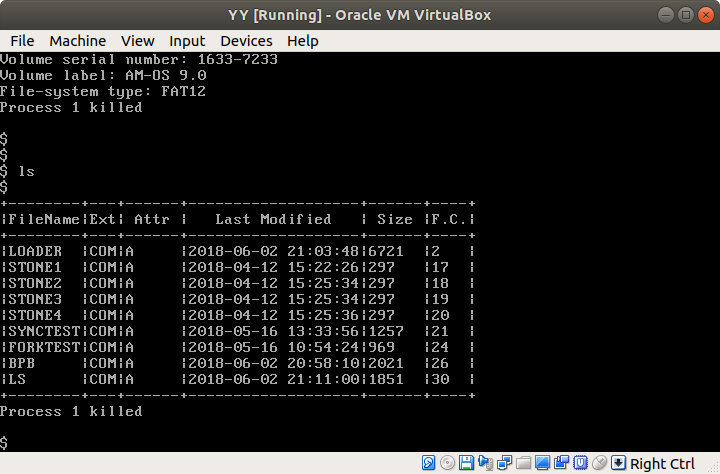
\includegraphics[scale=0.5]{pics/13.png}
\end{figure}

其中,LOADER.COM 为操作系统内核; STONE*.COM 为 4 个弹来弹去的用户程序;SYNCTEST.COM 为信号量测试程序;FORKTEST.COM 为 fork 测试程序;BPB.COM 为 BPB 显示程序; LS.COM 为显示根目录文件摘要的程序。

执行程序时,只需键入文件名(不含扩展名)即可。

\section{实验总结}

FAT12 分区本身并不复杂,但要弄清楚它,还是要花费一些时间的,最花时间的就是引导扇区程序了。由于很难在屏幕上显示调试信息,在写这个程序的时候,得不断地运行 bochs 来查看各个变量的值是否正确。

编写好引导扇区程序之后,我们只需要把操作系统内核、用户程序等等通过 Windows XP 复制到这个分区中即可,不再需要用 WinHex 来修改软盘啦!用 WinHex 修改软盘有多个弊端:有时删多了删少了导致软盘大小不等于 1.44 MB ,无法启动;有时把程序放错了位置。有了文件系统后,复制更方便了。我觉得文件系统这个实验应该在第三个实验(加载用户程序)之后立刻就做,以后的实验用上这个文件系统来复制用户程序就很方便。



\end{document}
















